\section{\I{Post processing output using \R} \label{sec:post-processing}}\index{Post processing}\index{Post processing section}

Hopefully when you get the bundle for this program there will be an \R\ package, this section describes how you can use that package to read in and view output from \IBM.  A list of the \R\ package functions are below.

\begin{itemize}
	\item \texttt{extract.run()} imports the model's output into the \R\ environment.
	\item \texttt{extract.ibm.file()} imports the model's configuration file into the \R\ environment as a list where you can change inputs. Useful in simulation based studies
	\item \texttt{write.ibm.file()} prints the a list object (that has the same characteristics as the \texttt{extract.ibm.file()})	to a text file.
	\item \texttt{reformat.compositional.data()} converts \IBM\ compositional observation reports into a more traditional matrix.
	\item \texttt{plot.derived\_quantities()} plot or extract derived quantities from a model run.
	\item \texttt{create\_ibm\_layer} A function that creates a file consists of \command{layer} block with a user input matrix, useful function for setting up highly spatial models.
	\item \texttt{csl2\_bio} turn a ibm biomass observation into a casal2 style observation
	\item \texttt{csl2\_fishery\_age} turn a ibm fishery age observation into a casal2 style observation	
	\item \texttt{csl2\_prop\_age} turn a ibm proportions at age observation into a casal2 style observation
	\item \texttt{ssb\_multiple\_runs} A plotting function to plot multiple Derived Quantities in ggplot style
	\item \texttt{plot\_numeric\_layer} a plotting function that generates a snapshot of biomass from a \subcommand{numeric\_layer} report. It generated the Figure~\ref{fig:pref}
\end{itemize}



Comparing different initialisation starts, as mentioned in the Tips section~\ref{sec:tips} we highly recommend that you reduce the initialisation phase as much as possible. Below is some \R\ code that I often use when looking at the effects of different initialisation phase burn-ins.

\begin{lstlisting}
library(ibm) ## for extracting
library(ggplot2) ## for plotting
library(reshape2) ## for reshaping data so its ggplot friendly

## read in a reported output from a ibm-r runs
## ---------------------------------
## An important note before running the models below.
## if you do not include the following report in your configuration files
##
## @report init_2
## type initialisation_partition
##
## this code will not work
## ---------------------------------
ibm_30 = extract.run("output_30.log")
ibm_50 = extract.run("output_50.log")
ibm_80 = extract.run("output_80.log")
ibm_120 = extract.run("output_120.log")

names(ibm_50)
mat = ibm_50$init_2$`1`$values

temp = rbind(ibm_30$init_2$`1`$values,ibm_50$init_2$`1`$values, ibm_80$init_2$`1`$values, ibm_120$init_2$`1`$values)
temp$burnin =  c(rep("30", nrow(mat)),rep("50", nrow(mat)), rep("80", nrow(mat)), rep("120", nrow(mat)))

merged = melt(temp)
colnames(merged) = c("cell", "burnin", "age", "frequency")

## plot age frequency for each row of spatial gird
for (i in 1:5) {
	temp_data = merged[substring(merged$`cell`,0,1) == as.character(i),]
	p <- ggplot(temp_data, aes(x = age, y = frequency, color = burnin)) + geom_point()
	p + facet_grid(cell ~ ., scales="free_y")
	print(p)
    Sys.sleep(2);
}
\end{lstlisting}

This should generate figures like in Figure~\ref{fig:initial_compare}

\vspace*{3mm}
\begin{figure}[htp]
	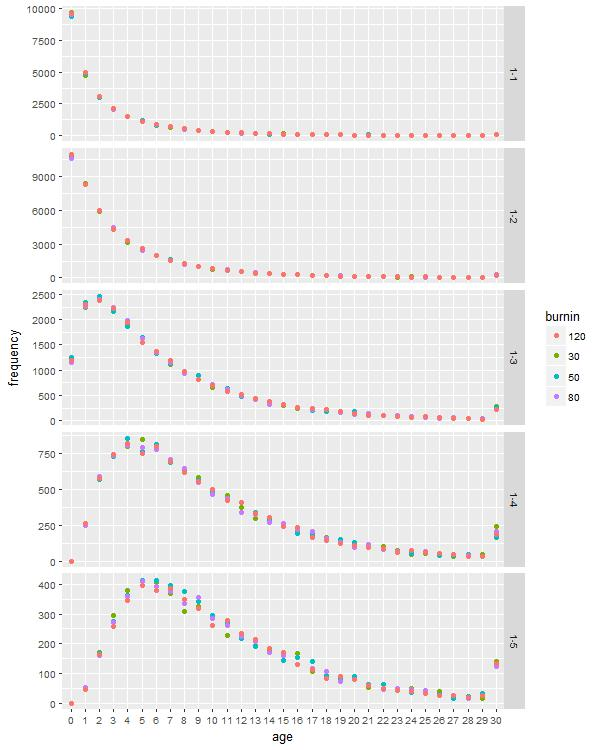
\includegraphics[scale=0.8]{Figures/Initial_age_comp_row_1.jpg}
	\caption{An example of plot that looks at the age frequency of different initial burn-in periods}\label{fig:initial_compare}
\end{figure}
